\section{Change report}
\subsection{Current situation}

In the orginal house.py file in the simulation folder, there is a function "scipy.integrate.odeint"  that calculates the ordinary differential equations from the domestic dwelling model. The SciPy website states however that this function should be replaced with scipy.integrate.solveivp. 

The code of the original ODE calculation in the house.py is as follows:

\begin{lstlisting}

for i in range(len(t)-1):

err = SP_T[i+1] - Tair[i]
Qinst = err * kp
Qinst = np.clip(Qinst, 0, 7000)

if (T_outdoor[i]>= 15):
Qinst=0
else:
Qinst=Qinst

inputs = (T_outdoor[i], Q_internal[i], Q_solar[i], SP_T[i], Qinst, CF,
Rair_outdoor, Rair_wall, Cair, Cwall)
# print(i)
ts = [t[i], t[i+1]]
y = odeint(model, y0, ts, args=inputs)

Tair[i+1] = y[-1][0]
Twall[i+1] = y[-1][1]
# integral[i+1]         = y[-1][2]

# Adjust initial condition for next loop

y0 = y[-1]
\end{lstlisting}

The way the odeint function is used in the original file is not correct. It is used in a for loop, in which only 2 points in time are used as input to calculate the state, in this case Tair and Twall. The output state that is generated in the iteration of the loop, is then used as intput for the next iteration. This causes unwanted oscillations in the output.

Control of the heat source 'Qinst' to control the indoor air temperature is also included in the for loop, however, it would be more beneficial to have the control part of the model inside the house model itself.

\subsection{Changes needed in the code to switch solver}

The routine can be improved by using the solve.ivp function from the Scipy library and removing the for loop.

The function has similar arguments, however, in the solve.ivp function, the y0 and time data are switched (see below).


\begin{lstlisting}
	#odeint example
	y = odeint(model, y0, ts, args=inputs)
	#solveivp example
	y = solve_ivp(model_buffervessel, [0, t[-1]], y0, args=inputs)
\end{lstlisting}

The inputs in the odeint function are single values. However, for the solve.ivp function an array is used for the inputs, since the inputs can change over time. An example is the setpoint of the indoor temperature. In the original file, the inputs changed with the help of the for loop, but the for loop will be removed with the solve.ivp function.

By incorporating the changes, the code snippet from the original file (see top of this document) can be replaced with the snippet below.

\begin{lstlisting}
inputs = (T_outdoor, Q_internal, Q_solar, SP_T, CF,
Rair_outdoor, Rair_wall, Cair, Cwall, UAradiator, Crad, Cbuffervessel, cpwater)
y = solve_ivp(model_buffervessel, [0, t[-1]], y0, args=inputs)
\end{lstlisting}

\subsection{Outcome comparison between the solvers}

Incorporating these changes will result in the following difference:

\begin{figure}[ht]
	\centering
	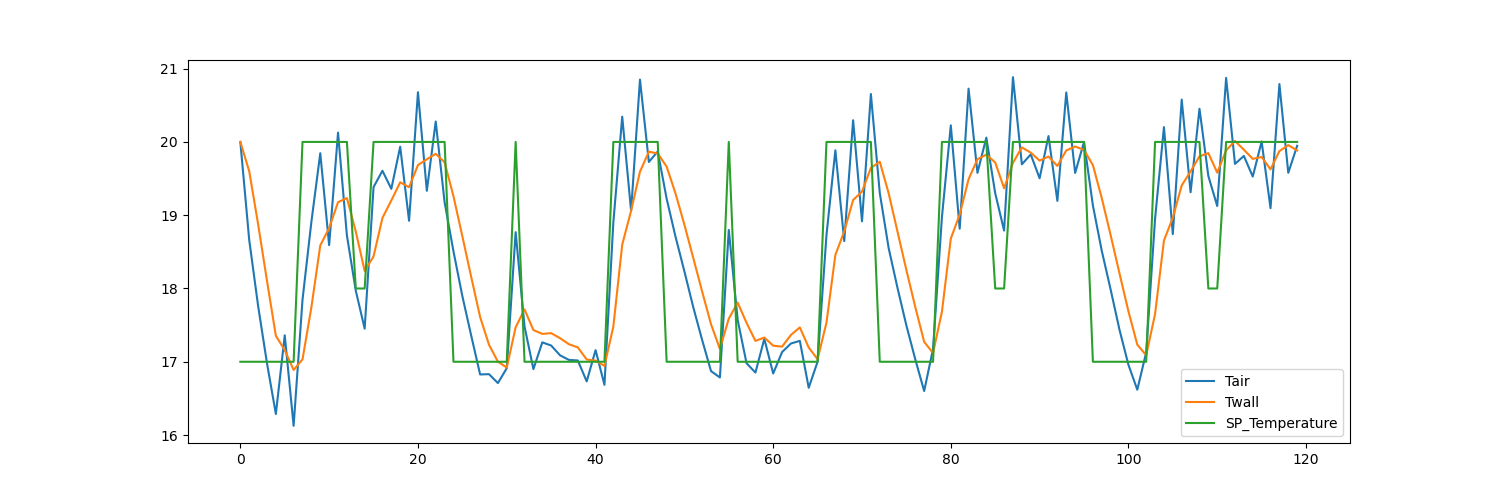
\includegraphics[width=1\columnwidth]{pictures/odeint_with_for_loop.png}
	\caption[Short title]{Indoor (wall)temperature output with ODEint}
	\label{fig:profilelabels}
\end{figure}

\begin{figure}[ht]
	\centering
	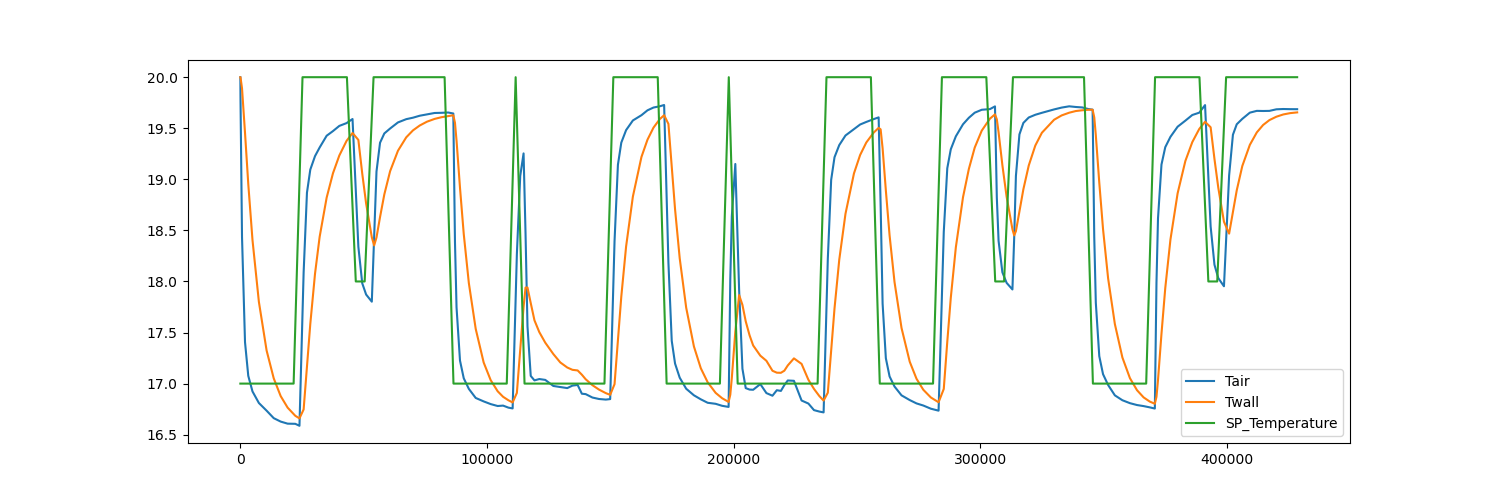
\includegraphics[width=1\columnwidth]{pictures/solve_ivp_without_for_loop.png}
	\caption[Short title]{Indoor (wall)temperature output with solve.ivp}
	\label{fig:profilelabels}
\end{figure}

As can be seen, a much smoother output is created by using the solve.ivp function.

	


